\documentclass[10pt,twocolumn,a4paper]{article}

\usepackage{amsfonts}
\usepackage{amsmath}
\usepackage{geometry}
\usepackage{xcolor,graphicx}
\usepackage[subfolder,cleanup]{gnuplottex}
%\usepackage{amsthm}
%\usepackage{enumitem}
%\usepackage{wrapfig}
\usepackage{subcaption}
%\usepackage{hyperref}
\usepackage{tikz}
\RequirePackage{cite}

\usetikzlibrary{patterns,decorations.pathreplacing}
\usetikzlibrary{arrows.meta}
\usetikzlibrary{shapes.arrows, fadings}

\let\originalleft\left
\let\originalright\right
\renewcommand{\left}{\mathopen{}\mathclose\bgroup\originalleft}
\renewcommand{\right}{\aftergroup\egroup\originalright}

\providecommand{\df}{\textrm{d}}
\newcommand{\diff}[3][\hspace{-0.5pt}]{\frac{\textrm{d}^{#1}#2}{\textrm{d}{#3}^{#1}}}
\newcommand{\pdiff}[3][\hspace{-0.5pt}]{\frac{\partial^{#1}#2}{\partial{#3}^{#1}}}
\newcommand{\Es}{E_{\textrm{sat}}}
\newcommand{\FT}[1]{\mathcal{F}\left\{ #1 \right\}}
\newcommand{\FTi}[1]{\mathcal{F}^{-1}\left\{ #1 \right\}}
\newcommand{\Her}[2]{\widetilde{H}_{#1} \left( #2 \right)}
\DeclareMathOperator{\sech}{sech}
%\newcommand{\eps}{\varepsilon}
%\newcommand{\rect}[1]{\textrm{rect}\left( #1 \right)}

\providecommand{\bigO}[1]{\ensuremath{\mathop{}\mathopen{}\mathcal{O}\mathopen{}\left(#1\right)}}

\newgeometry{margin=1.25cm}

\bibliographystyle{ieeetr}

\title{}
\author{B. Metherall \and C. S. Bohun}

\begin{document}

\twocolumn[
	\begin{@twocolumnfalse}
		\maketitle
		\begin{abstract}

		\end{abstract}
	\end{@twocolumnfalse}
]

\section{Introduction}
\label{sec:intro}
A tuneable laser has the ability to vary the frequency of its output by up to about 100 nanometres \cite{bohun2015, burgoyne2010, yamashita2009}. Tuneable lasers simultaneously lase at all frequencies within this bandwidth. This tuneability leads to applications such as optical coherence tomography \cite{bohun2015, burgoyne2014, yamashita2009}, coherent anti-Stokes Raman spectroscopy \cite{burgoyne2014}, deep tissue multi-photon microscopy \cite{chung2017, liu2017}, and diagnostics of ultrafast processes \cite{burgoyne2014, silfvast2004}. A typical tuneable ring laser cavity is shown in Figure \ref{fig:cavity}.

The nonlinearity causes several effects to arise within the laser cavity due to the interplay of dispersion, modulation, and the nonlinearity \cite{bohun2015, coen1997, lapre2019, shao2019, woodward2018}. The effect of most interest for this paper is optical wave breaking which causes the leading edge of a pulse to be red shifted, and the trailing edge blue shifted\footnote{In a normally dispersive optical fibre.} to the point that a shock is developed \cite{anderson1992, rothenberg1989a, rothenberg1989b, tomlinson1984, tomlinson1985}. The frequency shifts cause the pulse to become rectangular in the frequency domain with a linear chirp over most of the pulse. Wave breaking manifests from self-phase modulation (SPM) which is a direct effect of the nonlinearity in which the pulse interferes with itself. This interference generates new frequencies which induces the rectangular profile \cite{agrawal2013, mollenauer1980, woodward2018}. Modulation instablility is another effect that will be of interest that typically arises in the anomolous dispersion regime. However, in the presence of multiple pulses modulation instability can emerge in the normal dispersion regime as well through cross-phase modulation (XPM) and four-wave mixing (FWM) \cite{agrawal1987, agrawal1989, agrawal2013, haelterman1992}. Modulation instability causes a wave to break into short pulses, and can cause a laser to lose mode-locking \cite{agrawal1987, coen1997, haelterman1992}. Within a ring laser cavity wave breaking and modulation instability can become parasitic leading to an unstable and unsustainable pulse. This gives rise to the need of understanding the rich landscape of the parameter space, and determining design principles to guarantee the ring laser is stable and sustainable \cite{bohun2015, burgoyneemail, finot2008, lapre2019, woodward2018}.

\section{Modelling Efforts}
\label{sec:modelling}
The standard equation for studying nonlinear optics is the nonlinear Schr\"odinger equation (NLSE),
\begin{align}
	\pdiff{A}{z} &= - i \frac{\beta_2}{2}\pdiff[2]{A}{T} + i \gamma |A|^2 A.
	\label{eq:smallnlse}
\end{align}
Here $A = A(T, z) : \mathbb{R}^2 \mapsto \mathbb{C}$ is the complex pulse amplitude, $\beta_2 \in \mathbb{R}$ is the second order dispersion, and $\gamma \in \mathbb{R}$ is the coefficient of nonlinearity. In practice, the NLSE, \eqref{eq:smallnlse}, lacks a few key terms, thus, it is often generalized by adding amplification and loss\footnote{Occasionally higher order terms are added as well.}. These additions give the generalized nonlinear Schr\"{o}dinger equation (GNLSE) \cite{agrawal2013, bohun2015, finot2008, peng2018, shtyrina2017, yarutkina2013},
	\begin{align}
	\pdiff{A}{z} &= - i \frac{\beta_2}{2}\pdiff[2]{A}{T} + i \gamma |A|^2 A + \frac{1}{2}g(A) A - \alpha A,
	\label{eq:nlse}
\end{align}
where $g(A)$ is an amplifying term due to the gain, and $\alpha \in \mathbb{R}^+$ is the loss due to scattering and absorption.

\begin{figure}[tbp]
	\centering
	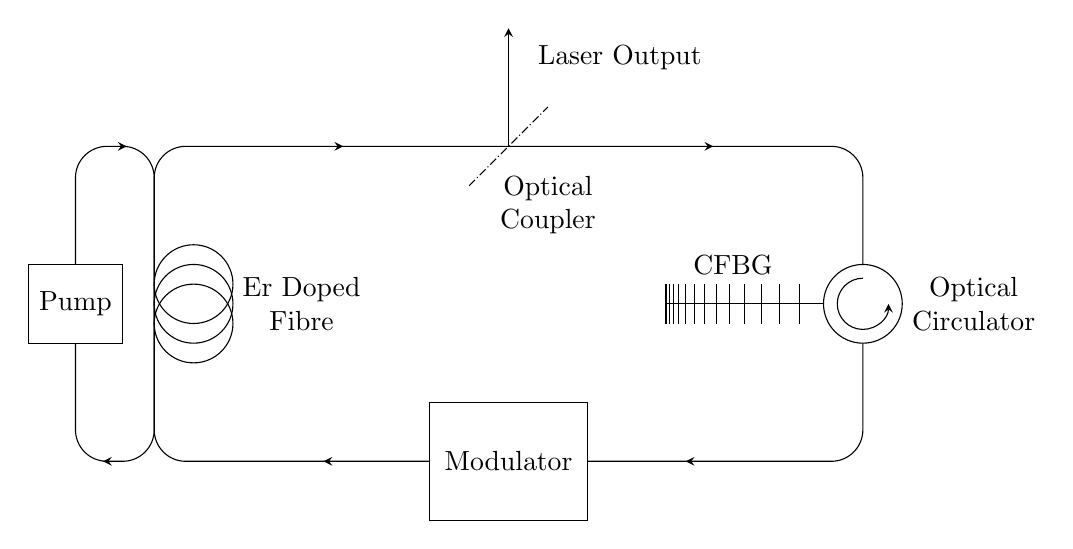
\begin{tikzpicture}
% Two laser loops
\draw [rounded corners=4mm] (0,0) rectangle ++(9,4);
\draw [rounded corners=4mm] (0,0) rectangle ++(-1,4);

% Gain
\draw (0.5,2.25) circle (0.5cm);
\draw (0.5,2) circle (0.5cm) node [anchor=west,xshift=0.5cm,align=center] {Er Doped \\ Fibre};
\draw (0.5,1.75) circle (0.5cm);

% Modulator and pump
\filldraw[fill=white, draw=black] (3.5,-0.75) rectangle ++(2,1.5) node [midway] {Modulator};
\filldraw[fill=white, draw=black] (-1.6,1.5) rectangle ++(1.2,1) node [midway] {Pump};

% Coupler and output
\draw[-stealth] (4.5,4) -- (4.5,5.5) node [pos=0.75,anchor=west,xshift=0.25cm] {Laser Output};
\draw[densely dashdotted] (4,3.5) -- (5,4.5) node [pos=1,anchor=north,yshift=-0.75cm,align=center] {Optical \\ Coupler};

% Circulator
\filldraw[fill=white, draw=black] (9,2) circle (0.5cm) node [anchor=west,xshift=0.5cm,align=center] {Optical \\ Circulator};
\draw[->,>=stealth] (9,2.325) arc (90:360:0.325cm);

% Grating
\draw (8.5,2) -- (6.5,2) node [pos=0.5,anchor=south,yshift=0.25cm,xshift=-0.15cm] {CFBG};
\foreach \i in {0,...,13}
  \draw (6.5 + \i*\i/100,1.75) -- (6.5 + \i*\i/100,2.25);

% Arrows
\draw[-stealth] (2.16,0) -- (2.15,0);
\draw[-stealth] (2.39,4) -- (2.4,4);
\draw[-stealth] (6.76,0) -- (6.75,0);
\draw[-stealth] (7.09,4) -- (7.1,4);
\draw[-stealth] (-0.649,0) -- (-0.65,0);
\draw[-stealth] (-0.351,4) -- (-0.35,4);H
\end{tikzpicture}
	\caption{Typical cavity of a fibre ring tuneable laser \cite{burgoyne2014, chung2017, lapre2019, shao2019, tang2014}. The laser pulses travel clockwise around each loop.}
	\label{fig:cavity}
\end{figure}

The GNLSE has many applications in nonlinear optics and fibre optic communications, however, in laser physics typically a modulation term is also added to ensure mode-locking, this yields the master equation of mode-locking \cite{haus1984, haus1975, haus1986, haus1992, haus2000, tamura1996, usechak2005},
\begin{align}
	\pdiff{A}{z} &= - i \frac{\beta_2}{2}\pdiff[2]{A}{T} + i \gamma |A|^2 A + \frac{1}{2}g(A) A - \alpha A - M(T).
	\label{eq:meml}
\end{align}
No analytic solution is known for \eqref{eq:meml}---even after making the assumptions that the gain is constant, and the modulation is quadratic \cite{haus1984, haus1975, haus1996}. However, by neglecting certain terms of \eqref{eq:meml} analytic solutions can be found \cite{burgoyne2014, haus1975, haus1986, haus1991, haus1992, haus1996, tamura1996, usechak2005}. Furthermore, see Haus \cite{haus2000} for a comprehensive description and history of the theory of mode-locked lasers.

\subsection{Discrete Models}
\label{sec:discrete}
Unfortunately, the master equation, \eqref{eq:meml}, is not completely representative of the underlying physics within our laser cavity. In the derivation of \eqref{eq:meml} it is assumed each process affects the pulse continuously within the cavity. As highlighted by Figure \ref{fig:cavity}, this can be a poor assumption. Within the cavity, each effect is localized to its corresponding component: almost all of the dispersion happens within the chirped fibre Bragg grating (CFBG) \cite{agrawal2002}, the pulse is only amplified within the Erbium-doped fibre, etc. Thus, a better model is one where \eqref{eq:meml} is broken down into the individual components giving the effect of each `block' of the cavity. Each of the blocks can then be functionally composed together to give an iterative map for the effect of one round trip of the cavity. This ultimately transforms the differential equation into an algebraic equation.

Such a method was first proposed in 1955 by Cutler \cite{cutler1955} while analyzing a microwave regenerative pulse generator. This method was adapted for mode-locked lasers in 1969 by Siegman and Kuizenga \cite{kuizenga1970a, kuizenga1970b, kuizenga1970, siegman1969}. The effects of the nonlinearity would not be considered until Martinez, Fork, and Gordon \cite{martinez1984, martinez1985} tried modelling passively mode-locked lasers. This issue has recently been readdressed by Burgoyne \cite{burgoyne2014} in the literature for tuneable lasers. In each of these models the effect of each block is described by a transfer function.

Despite the development of these block style models, several short-comings exist. The clearest is that none of these models have contained every block---either the nonlinearity or the modulation have been omitted. Each component of a tuneable plays a crucial role and the laser will not function correctly without the inclusion of all of the components. Another drawback is that the functional operations of some of the components used in their models are phenomenological. While these functions are chosen based on the observed output, they are not necessarily consistent with the underlying physics. Finally, none of these previous models have been able to exhibit wave breaking.


\section{Model Derivation}
\label{sec:model}
Using the idea of a discrete model presented Section \ref{sec:discrete}, we derive our model from the GNLSE, \eqref{eq:nlse}; however, in the case of the modulation we consider the exact functional form to be determined by the laser operator. To accomplish this, we neglect all terms but one of the right side of \eqref{eq:nlse} and solve the simplified differential equation. This is a reasonable assumption since the gain, loss, dispersion, modulation, and nonlinear effects are localized to only one section of the laser cavity.

To proceed we must choose the form of the amplification term, $g(A)$. We assume the gain has the form
\begin{align}
	g(A) &= \frac{g_0}{1 + E / \Es},& E &= \int_{-\infty}^\infty |A|^2 \, \df T,
	\label{eq:energy}
\end{align}
where $g_0$ is a small signal gain, $E$ is the energy of the pulse, and $\Es$ is the energy at which the gain begins to saturate \cite{bohun2015, burgoyne2014, haus1975, haus1984, haus1992, haus2000, haus1991, kartner2005, peng2018, shtyrina2017, silfvast2004, usechak2005, yarutkina2013}. This leads to
\begin{align}
	G(A) &= \left( \frac{\Es}{E} W \left( \frac{E}{\Es} \textrm{e}^{E/\Es} \textrm{e}^{g_0 L_g} \right) \right)^{1/2} A
\end{align}
for the amplification of the pulse within the Er-doped fibre. Continuing this process for the loss, dispersion, and nonlinearity yields
\begin{align}
	L(A) &= (1 - R) \textrm{e}^{- \alpha L_T}A, \\
	D(A) &= \FTi{\textrm{e}^{i \omega^2 L_D\beta_2/2} \FT{A}}, \\
	F(A) &= A \textrm{e}^{i \gamma |A|^2 L_f},
\end{align}
where $R$ is the reflectivity of the output coupler\footnote{Depending on the layout of the laser cavity the loss may instead take the form $L(A) = R \textrm{e}^{- \alpha L_T}A$.}, $L_T$ is the total length of the laser circuit, $L_D$ is the length of the dispersive medium, $L_f$ is the length of fibre between the amplifier and the output coupler, and where $\mathcal{F}$ denotes the Fourier transform. Finally, we must assume a form for the modulation. The modulation is considered to be applied externally in which ever way the operator sees fit. For simplicity the representation is taken as the Gaussian
\begin{align}
	M(A) &= \textrm{e}^{-T^2 / 2 T_M^2} A,
	\label{eq:modform}
\end{align}
where $T_M$ is the characteristic width of the modulation. This assumption is not particularly restrictive. Calcaterra and Boldt have shown that Gaussians can form a basis for $L^2(\mathbb{R})$ \cite{calcaterra2008a}. Therefore, we can approximate any modulation function in $L^2(\mathbb{R})$ by a sum of \eqref{eq:modform}.

\subsection{Non-Dimensionalization}
The structure of each process of the laser can be better understood by re-scaling the time, energy, and amplitude; this suggests the convenient scalings:
\begin{align}
	T &= T_M \widetilde{T},& E &= \Es \widetilde{E},& A &= \left( \frac{\Es}{T_M} \right)^{1/2} \widetilde{A}.
\end{align}
Revisiting each process map shows each process has a characteristic non-dimensional parameter. The new mappings---after dropping the tildes---are
\begin{equation}
	\begin{aligned}
		G(A) &= \left(E^{-1} W \left( a E \textrm{e}^{E}\right) \right)^{1/2} A, & F(A) &= A \textrm{e}^{i b |A|^2}, \\
		D(A) &= \FTi{\textrm{e}^{i s^2 \omega^2} \FT{A}}, & L(A) &= h A, \\
		M(A) &= \textrm{e}^{-T^2 / 2} A,
		\label{eq:effects}
	\end{aligned}
\end{equation}
with the four dimensionless parameters,
\begin{equation}
	\begin{aligned}
		a &= \textrm{e}^{g_0 L_g} \sim 8 \times 10^3,& \qquad h &= (1 - R) \textrm{e}^{-\alpha L} \sim 0.04, \\
		b &= \gamma L_f \frac{\Es}{T_M} \sim 1,& \qquad s &= \sqrt{\frac{\beta_2 L_D}{2 T_M^2}} \sim 0.2,
		\label{eq:ndparam}
	\end{aligned}
\end{equation}
which characterize the behaviour of the laser. Nominal values for the parameters, \eqref{eq:ndparam}, can be found in \cite{agrawal2002, agrawal2013, bohun2015, burgoyne2014, burgoyneemail, finot2008, li1998, litchinitser1997, peng2018, shtyrina2017, tamura1993, tamura1996, tomlinson1984, usechak2005, yamashita2009, yarutkina2013}. Notice that the modulation is only characterized by $T_M$, and each other process has its own associated independent non-dimensional parameter.

% Table of parameter values
% \begin{table*}[tbp]
% 	\centering
% 	\begin{tabular}{lcll}
% 		\hline\noalign{\smallskip}
% 		Parameter & Symbol & Value & Sources \\
% 		\hline\noalign{\smallskip}
% 		Absorption of Fibre & $\alpha$ & $10^{-4}$--$0.3\text{ m}^{-1}$  & \cite{burgoyneemail, shtyrina, tomlinson, usechak, yarutkina} \\
% 		Fibre Dispersion & $\beta_2^f$ & $-50$--$50 \text{ ps}^2/ \text{km}$ & \cite{agrawal2002, agrawal2013, burgoyne2014, litchinitser, peng, yarutkina} \\
% 		Fibre Nonlinearity & $\gamma$ & $0.001$--$0.01 \text{ W}^{-1} \text{m}^{-1}$ & \cite{agrawal2013, finot, usechak, yarutkina} \\
% 		Grating Dispersion & $\beta_2^g L_D$ & $10$--$2000 \text{ ps}^2$ & \cite{agrawal2002, agrawal2013, burgoyne2014, li} \\
% 		Length of Cavity & $L_T$ & $10$--$100 \text{ m}$ & \cite{burgoyneemail, peng, tamura1996} \\
% 		Length of Fibre & $L_f$ & $0.15$--$1 \text{ m}$ & \cite{burgoyneemail} \\
% 		Length of Gain Fibre & $L_g$ & $2$--$3 \text{ m}$ & \cite{burgoyne2014, peng, shtyrina, tamura1993, yarutkina} \\
% 		Modulation Time & $T_M$ & $15$--$150 \text{ ps}$ & \cite{bohun, burgoyneemail, burgoyne2014} \\
% 		Reflectivity of Optical Coupler & $R$ & $0.1$--$0.9$ & \cite{burgoyneemail, li, peng,  tamura1993, tamura1996, yamashita} \\
% 		Saturation Energy & $\Es$ & $10^3$--$10^4 \text{ pJ}$ & \cite{burgoyneemail, usechak, yarutkina} \\
% 		Small Signal Gain & $g_0$ & $1$--$10 \text{ m}^{-1}$ & \cite{burgoyneemail, yarutkina} \\
% 		\noalign{\smallskip}\hline
% 	\end{tabular}
% 	\caption{Range of variation of various parameters.}
% 	\label{tab:values}
% \end{table*}

\subsection{Combining the Effects}
\label{sec:effects}

\begin{figure}[tbp]
	\centering
	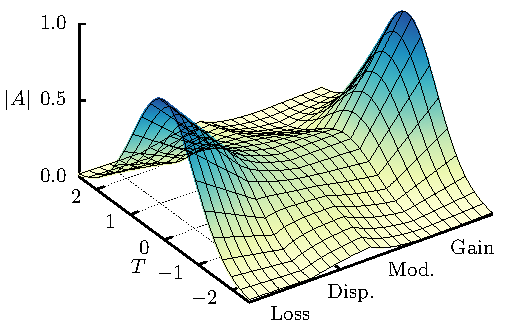
\includegraphics{Evo}
	\caption{Evolution of the envelope during one round trip of the cavity at equilibrium. The pulse decays due to the output coupler, dispersed by the CFBG, modulated by the modulator, and finally amplified by the gain fibre (the envelope is unaltered by the nonlinearity). Note that this is for visualization only, the durations are not to scale.}
	\label{fig:cavityevo}
\end{figure}

Now that we have the algebraic effect of each section of the cavity, we are ready to compose each map together to give the effect of one round trip of the cavity. Thus, we must now consider the order of the components. As we are most interested in the output of the laser cavity, we shall start with the loss. We then pass the pulse through the CFBG followed by the modulator. The pulse then travels through the Er-doped fibre to be amplified, and finally we consider the effect of the nonlinearity. The nonlinearity must immediately follow the gain---this is the section of the cavity where the pulse is most energetic, and hence, has the largest effect. Note, the permutation of the other components is indeed important as the operators do not, in general, commute---this is in contrast to the models described in Section \ref{sec:discrete}. Moreover, we prefer the loss to follow the gain and nonlinearity as we wish to minimize the length over which the nonlinearity has an effect, and maximize the output power. Functionally we denote one round trip of the cavity by
\begin{align}
	\mathcal{L}(A) = F(G(M(D(L(A))))).
\end{align}
 The pulse after one complete circuit of the laser cavity is then returned back into the cavity to restart the process. A steady solution to this model is one in which the envelope and chirp are unchanged after traversing every component in the cavity---we are uninterested in the phase. That is, such that $\mathcal{L}(A) = A \textrm{e}^{i \phi}$---for some $\phi \in \mathbb{R}$. In Figure \ref{fig:cavityevo} we can see an example of the evolution of the envelope of the pulse during one round trip of the cavity.

\section{Results}
We split the results into two subsections. In the following subsection we investigate the low nonlinearity limit, and in Section \ref{sec:nlresults} we look at the full nonlinear model.

\subsection{Linear Solution}
By neglecting the effect of the nonlinearity, that is, $b = 0$, a solution can be found analytically. We assume the solution will take the form of a chirped Gaussian. There are a few reasons for this; the solution to the models presented in \cite{cutler1955, siegman1969, kuizenga1970a, martinez1984, martinez1985} were Gaussian, the equilibrium shape will be highly correlated to the shape of the modulation function, and since a Gaussian is a fixed point of the Fourier transform \cite{gradshteyn2007}. Furthermore, this form is chosen because it resembles the envelope and linear chirp expected \cite{burgoyne2014, haus1975, haus1996, haus2000, usechak2005}.

To compute $\mathcal{L}(A)$, consider the pulse
\begin{align}
	A = \sqrt{P} \exp \left( -(1 + iC) \frac{T^2}{2 \sigma^2} \right) \textrm{e}^{i \phi_0},
	\label{eq:A0}
\end{align}
where $P$ is the peak power, $C$ is the chirp, $\sigma^2$ is the variance, and $\phi_0$ is the initial phase. This pulse shape is depicted in Figure \ref{fig:samplegauss}.

\begin{figure}[tbp]
	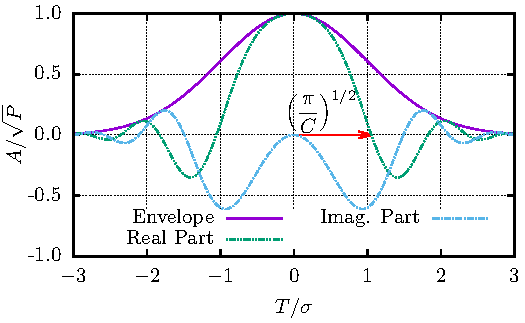
\includegraphics{Sample_Gauss}
	\caption{Solution to the linear model given by \eqref{eq:A0}.}
	\label{fig:samplegauss}
\end{figure}

To compute $\mathcal{F}(A)$, given the initial pulse \eqref{eq:A0}, we iteratively compute the effect of each process map from \eqref{eq:effects}. Now, by equating $\mathcal{F}(A)$ and $A \textrm{e}^{i \phi}$ we obtain a system of equations. In particular,
\begin{gather}
	\sigma^8 + 4 s^4 \sigma^6 - 20 s^4 \sigma^4 + 32 s^4 \sigma^2 - 16 s^4 = 0, \label{eq:var} \\
	C = \frac{\sigma^4 \pm \sqrt{\sigma^8 - 16 s^4 \left( 1 - \sigma^2 \right)^2}}{4 s^2 \left( 1 - \sigma^2 \right)}.
	\label{eq:chirp}
\end{gather}

As \eqref{eq:var} is a quartic in $\sigma^2$ it has an analytic solution, namely,
\begin{equation}
	\begin{split}
		\sigma^2 = \sqrt{2} s \left( s^6 + 3s^2 + \sqrt{4 + s^4} \left( 1 + s^4 \right) \right)^{1/2} & \\
		- s^4 - s^2 & \sqrt{4 + s^4},
		\label{eq:equilvar}
	\end{split}
\end{equation}
which can readily be used to find the chirp, $C$. By asymptotically expanding \eqref{eq:var} we find the useful relations
\begin{align}
	\sigma^2 &\sim
	\begin{cases}
		2s(1 - s) + \bigO{s^3} & s \rightarrow 0 \\
		1 - \frac{1}{4}s^{-4} + \frac{3}{8}s^{-8} + \bigO{s^{-12}} & s \rightarrow \infty,
	\end{cases} \\
	C &\sim
	\begin{cases}
		1 - s + \frac{1}{2}s^2 + \bigO{s^3} & s \rightarrow 0 \\
		\frac{1}{2}s^{-2} - \frac{3}{8}s^{-6} + \bigO{s^{-10}} & s \rightarrow \infty.
	\end{cases}
\end{align}
The equilibrium energy and peak power can be found by conservation of energy to give
\begin{align}
	E = \frac{h^2 \left( 1 - \sigma^2 \right)^{1/2}}{1 - h^2 \left( 1 - \sigma^2 \right)^{1/2}} \log \left( a h^2 \left( 1 - \sigma^2 \right)^{1/2} \right),
\end{align}
and
\begin{align}
	P = \frac{W(a E \textrm{e}^E)}{\sqrt{\pi} \sigma},
	\label{eq:equilpower}
\end{align}
respectively.

Our linearized model indeed exhibits the same form as previous linear models. However, by including the effects of the nonlinearity we uncover the rich interplay between dispersion, modulation, and nonlinearity not previously found mathematically.

\subsection{Nonlinear Solution and Instability}
\label{sec:nlresults}

In this iterative scheme---as well as within the laboratory---we must specify the input pulse shape. The most common form is a hyperbolic secant \cite{coen1997, finot2008, mitschke1986, rothenberg1989b, tomlinson1984}, which we assume has the exact form
\begin{align}
	A_0 = \Gamma \sech \left( 2 T \right) \textrm{e}^{i \pi / 4},
\end{align}
where $\Gamma$ is a normalizing factor chosen so the pulse has an initial energy of $E_0 = 0.1$.



xpm \cite{agrawal2013, agrawal1987, agrawal1989}



\begin{figure}[tb]
	\centering
	\begin{subfigure}{\columnwidth}
		\centering
		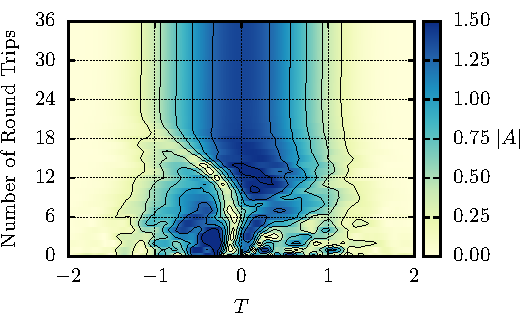
\includegraphics{Conv}
		\caption{Example of a pulse stabilizing from a seemingly random initial pulse shape ($s = 0.1$, $b = 1.0$, $E_0 = 0.1$, $a = 8000$, $h = 0.04$).}
		\label{fig:convevo}
	\end{subfigure} \\
	\begin{subfigure}{\columnwidth}
		\centering
		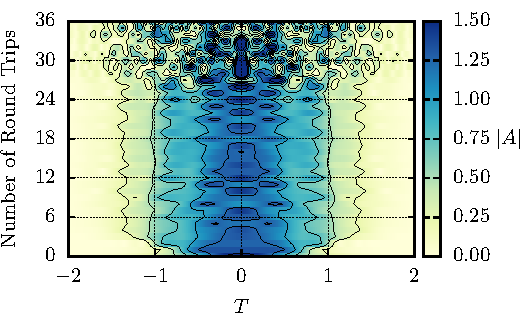
\includegraphics{Break}
		\caption{Example of a pulse destabilizing from a hyperbolic secant initial pulse ($s = 0.1$, $b = 1.6$, $E_0 = 0.1$, $a = 8000$, $h = 0.04$).}
		\label{fig:breakevo}
	\end{subfigure}
	\caption{Two extremes of the evolution of a pulse.}
	\label{fig:evolution}
\end{figure}



\begin{figure}[tbp]
	\centering
	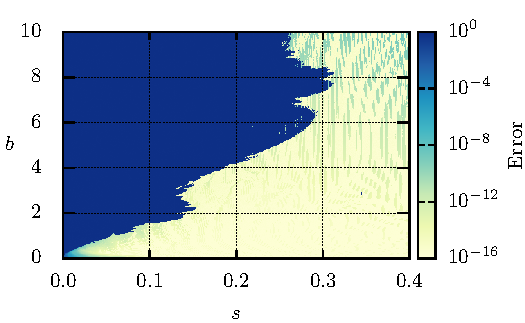
\includegraphics{ParamSpaceErr}
	\caption{}
	\label{fig:error}
\end{figure}

\begin{figure}[tbp]
	\centering
	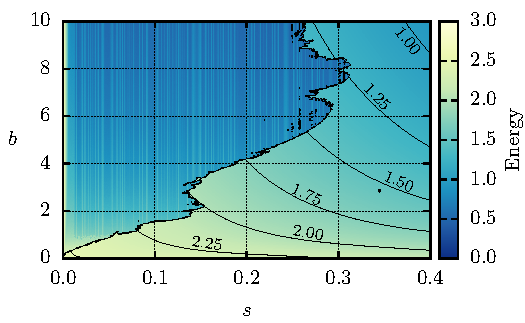
\includegraphics{ParamSpaceEnergy}
	\caption{}
	\label{fig:}
\end{figure}



\begin{figure}[tbp]
	\centering
	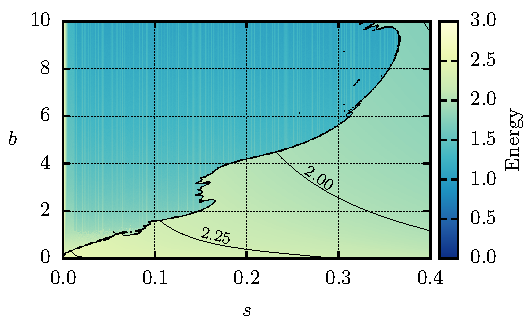
\includegraphics{ParamSpaceEnergySwitch}
	\caption{}
	\label{fig:energyswitch}
\end{figure}


\section{Conclusion}


\clearpage
\newpage




\section{Nonlinear Solution}
We now consider the nonlinear case---when $b > 0$. In this case it becomes impossible to obtain an analytic result. Recall from \eqref{eq:effects} that the nonlinearity is a highly nonlinear operator, and attempting to compute the Fourier transform analytically of a pulse that has undergone this transformation is futile. Instead we resort to a numerical solution.

With the inclusion of the nonlinearity we generally find a similar solution to the linear case. An example of this is shown in Figure \ref{fig:nlstable}.

Instead, the magnitude of the Fourier transform has a unique weakly bi-modal shape. This deviation suggests the nonlinearity implants higher frequency oscillations into the pulse---a key observation in the coming subsections. Finally, we shall examine the derivative of the phase---essentially the chirp.

 In the nonlinear case, we recover this linear response for moderate values of $T$. However, for $|T| > 1$ the chirp begins to saturate. This is consistent with the experimental results \cite{chen, rothenberg, tomlinson}.


The noise in the energy exhibited for moderate to large values of $b$, and small values of $s$ is a phenomenon called \emph{wave breaking} \cite{agrawal2013, anderson, finot, rothenberg, tomlinson}. Wave breaking is not limited to just optics; wave breaking occurs in areas such as plasmas, transmission lines, and fluid dynamics \cite{rothenberg}. Wave breaking occurs because the pulse begins to interfere with itself in a way called SPM \cite{agrawal2002, agrawal2013, becker}. SPM occurs because the index of refraction is intensity dependent \cite{agrawal2002, becker, rothenberg, silfvast}, which leads to additional chirp across the pulse \cite{agrawal2013, anderson, rothenberg, silfvast}. This in turn causes higher order frequencies to be injected into the pulse \cite{agrawal2013, anderson}, as we saw in Figure \ref{fig:nlstable}. These high frequencies compound with each trip around the cavity becoming parasitic very quickly---Figure \ref{fig:break} highlights this. Notice that the difference between Figure \ref{fig:nlstable} and Figure \ref{fig:break} is a difference in $b$ of $0.05$---just enough to cross the boundary---this difference could be attributed to adding a few centimetres more of fibre between the gain and output coupler. \\

The left figures show the pulse after 11 trips around the cavity; in the Fourier transform it is clear that the contributions from higher frequencies has increased. We obtain comparable results as in the experiments \cite{anderson, rothenberg}. Additionally, the chirp starts losing its linearity causing it to start becoming unstable; the nature of this instability is again in agreement with the experiments \cite{anderson, rothenberg}. The parasitic nature of the high frequency contributions is evident by examining the right figures. After five additional trips around the cavity, the envelope of the pulse is much more rippled, and the real and imaginary parts become incoherent. Moreover, the Fourier transform has no clear structure and has essentially become noise. The chirp has grown to be highly oscillatory and unstable. Once the pulse has reached a state such as this, the envelope, Fourier transform, and chirp never reach a steady equilibrium state.




To obtain a better understanding of how the pulse either converges to equilibrium, or diverges to wave breaking, we shall examine the difference between the envelopes of consecutive iterations. More precisely, we compute the error by
\begin{align}
	\textrm{E} = \frac{\| |A_i| - |A_{i-1}| \|_2}{\| A_{i-1} \|_2},
	\label{eq:error}
\end{align}
where $\| \cdot \|_2$ denotes the $L^2(\mathbb{R})$ norm, which is computed numerically using the trapezoid rule ($N = 2^{18}$). Notice as well that in the numerator we use the modulus of the pulses, again this is because we are uninterested in the phase shift between iterations. A plot of the error can be found in Figure \ref{fig:error}, with $i = 100$. The standard method would be to iterate until a fixed tolerance is reached, however, there are some reasons that make a fixed number of iterations preferable---as long as a sufficient number is chosen. The main reason is that this allows us to observe a richer structure than simply whether or not the tolerance had been reached by some maximum number of iterations. Additionally, incorrectly choosing the critical tolerance could easily lead to erroneous categorizations at points.

Unsurprisingly, the error is largest in the region where the wave breaks. As mentioned in the previous subsection, the pulse does not reach a stable state in this region. As a consequence the envelope varies drastically, which leads to this large error.




The last item we wish to consider is the order in which the components are placed. In Section \ref{sec:effects} a brief description for the choice of the order was given. We start with the loss component since this coincides with the output; the fibre nonlinearity follows the gain since this is where it has the largest impact; and the loss follows the nonlinearity in an attempt to mitigate its effect. Therefore, the loss is first, and the gain followed by the nonlinearity are last---leaving dispersion and modulation in the middle. We chose to put the dispersion block ahead of the modulator. However, there was no real reason behind this---modulation before dispersion is equally as valid---and in this subsection we explore the effect of modulating the pulse before it passes through the CFBG. \\

The result of this switch is shown in Figure \ref{fig:switch}. As a whole, unsurprisingly, we find the same behaviour and structure, however, there are some intriguing differences. Again, the structure and periodic nature of the boundary is similar to before, however, this boundary has shifted rightwards to a larger $s$ value. Additionally, within the unstable region the density of the contour lines is much greater---suggesting it is in some sense more chaotic and random than with the components in their original permutation. The final main difference between the two orderings, is that in this case the energy contours are no longer monotonic functions of $s$. Instead we find a parabolic shape on the top contour, and two lobes on the second contour. \\






\section{Conclusion}
Within this paper we developed a new nonlinear model for tuneable lasers. In order to better represent the underlying physics within the laser cavity the nonlinear Schr\"{o}dinger equation was reduced to simpler differential equations for each component of the laser. This led to a functional map that defines the effect of each component on a particular input pulse. These processes were then composed together to give an iterative mapping of the whole laser cavity. In a future publication we shall show the results obtained by this iterative mapping as well as discuss the dynamics exhibited by this model---including wave-breaking---to predict the conditions under which the pulse is stable and sustainable.


\bibliography{Ref}

\end{document}
